\chapter{Planejamento do projeto}

  Para o planejamento do projeto foi definido um cronograma com todas as atividades, data de entrega, recursos, e integrantes que irá
  realizar determinada tarefa, mantendo sempre o controle dos entregaveis e do tempo para finalizar o projeto.

\section{Cronograma}

  A elaboração do cronograma se deu na ferramenta do Gantter para google driver, o cronograma será dividido em trabalho 1 e 2,
  na qual será feito e aprimorada no decorrer do semestre, a primeira entrega, trabalho 1, se refere ao planejamento,
  definição da abordagem, processos, ferramentas e técnicas de elicitação de requisitos. A segunda se refere a evolução e execução
  do processo estipulado, levantamento dos requisitos e planejamento e execução das sprints e releases.

  A figura abaixo ilustra o cronograma da equipe no trabalho 1.

  \begin{figure}[!h]
    \centering
    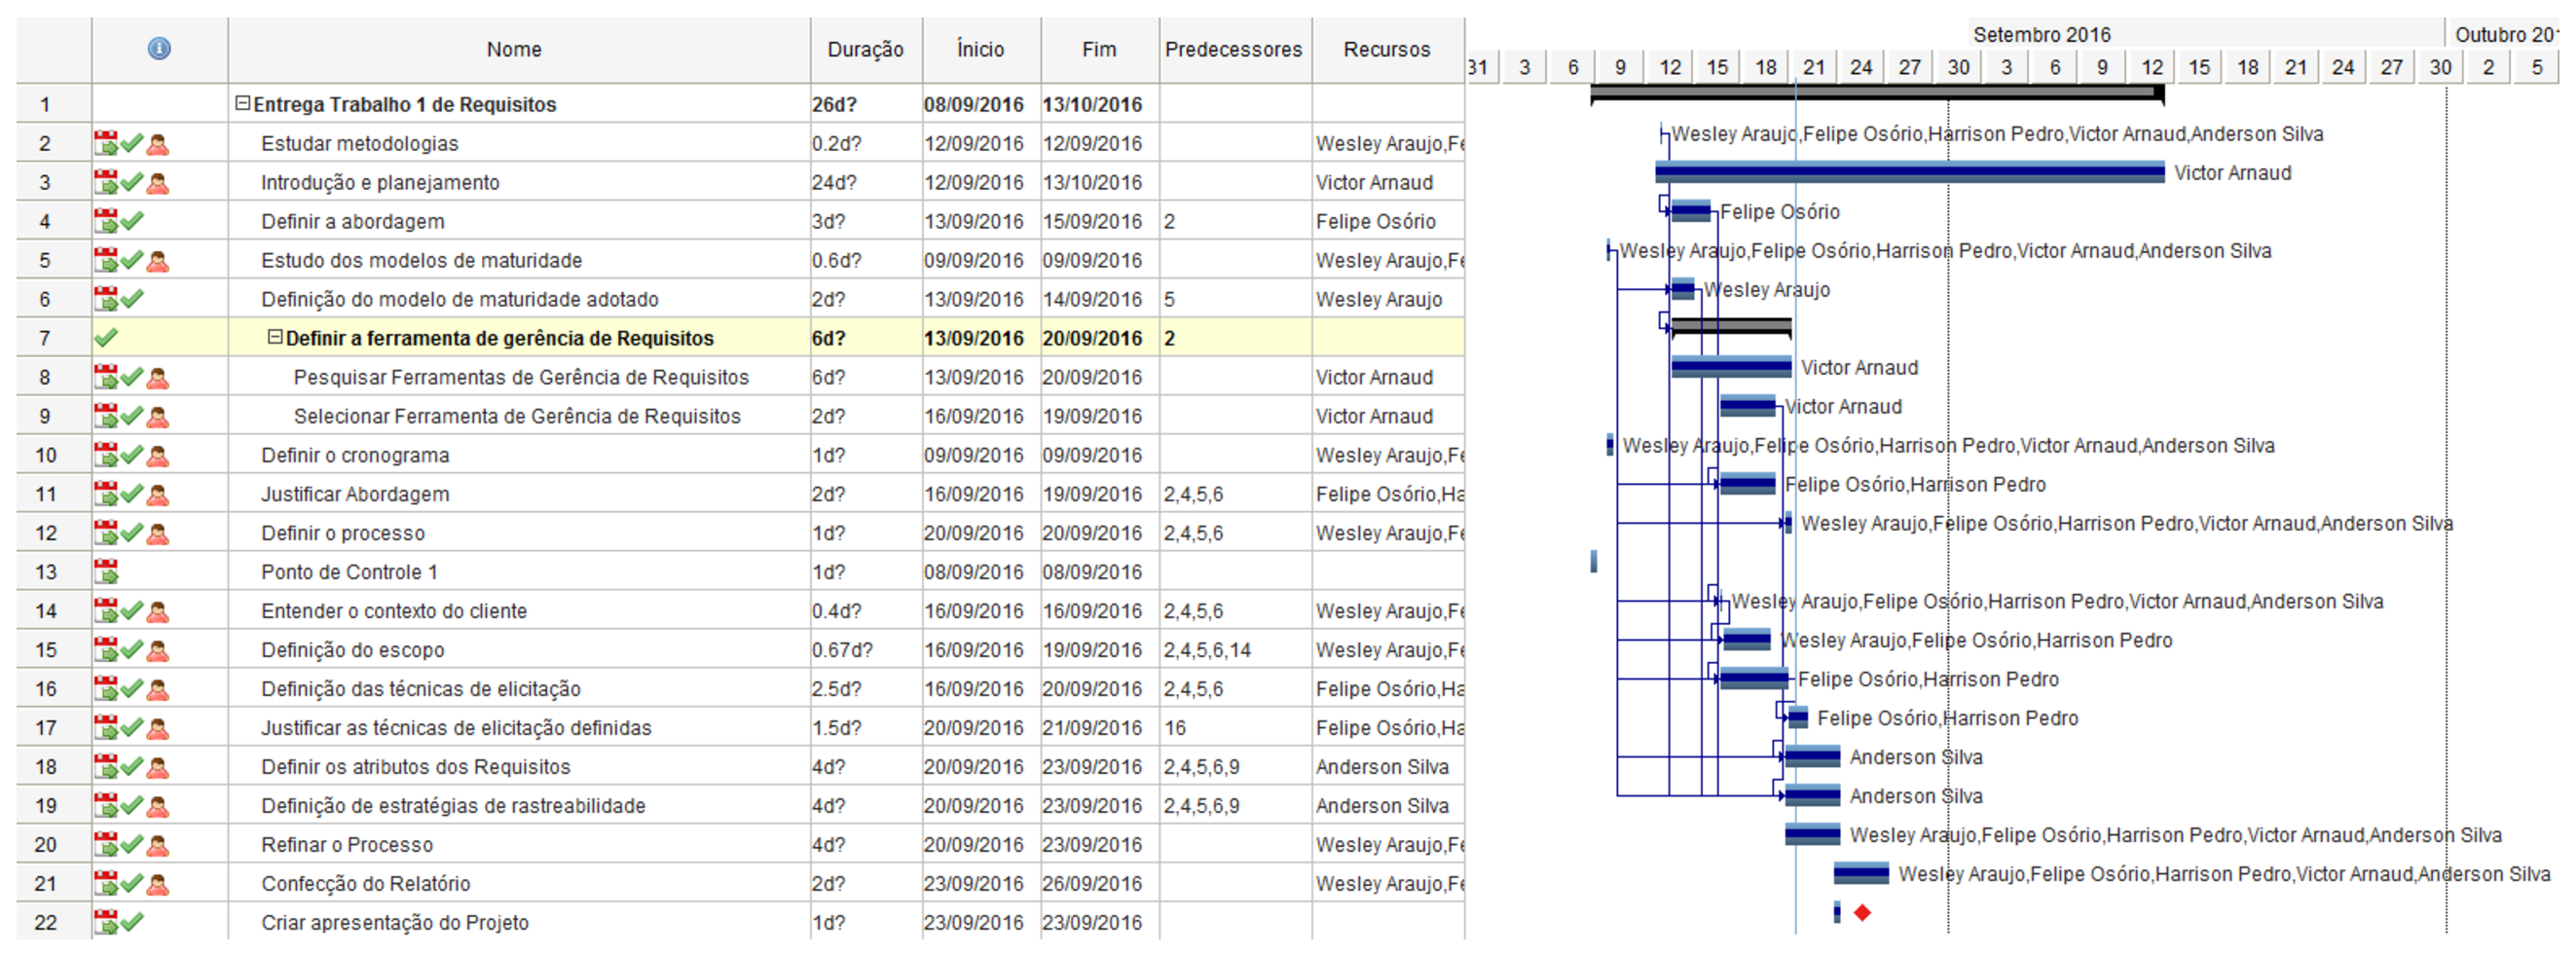
\includegraphics[width=15cm, keepaspectratio=true]{figuras/cronograma/cronograma.eps}
    \caption{Cronograma}
  \end{figure}

